% CHƯƠNG 4: KẾT QUẢ THỰC NGHIỆM VÀ ĐÁNH GIÁ
% =====================================================================
\chapter{KẾT QUẢ THỰC NGHIỆM VÀ ĐÁNH GIÁ}
\label{chap:ket-qua}

Chương 4 trình bày các kết quả thực nghiệm thu được từ hệ thống đề xuất và so sánh với các phương pháp nén truyền thống H.264/AVC và H.265/HEVC. Nội dung được tổ chức thành tám phần. Phần đầu mô tả thiết lập thực nghiệm. Phần thứ hai đánh giá hiệu năng của mô-đun phân đoạn dựa trên PIDNet-L. Phần thứ ba phân tích chất lượng tái tạo theo các thước đo truyền thống. Phần thứ tư đánh giá theo các thước đo nhận thức ngữ nghĩa. Phần thứ năm phân tích tác động của hệ thống lên tác vụ phân đoạn hạ nguồn. Phần thứ sáu đánh giá chiến lược điều khiển CRF thích nghi RA-CRF. Phần thứ bảy đánh giá tốc độ xử lý end-to-end. Phần cuối thảo luận và kết luận chương.

\section{Cơ sở thực nghiệm}
\label{sec:thiet-lap}

\subsection{Các kết quả đánh giá thực nghiệm}
\label{subsec:baseline}

Bốn kết quả
 được so sánh trong thực nghiệm. Thứ nhất là H.264/AVC tiêu chuẩn sử dụng bộ mã hóa x264 với CRF cố định, không có cơ chế phân biệt vùng. Thứ hai là H.265/HEVC tiêu chuẩn sử dụng bộ mã hóa x265 với CRF cố định, cũng không phân biệt vùng. Hai phương diện này đóng vai trò đường cơ sở để đánh giá lợi ích của việc áp dụng cơ chế phân vùng. Thứ ba là hệ thống SAC dùng mô hình phân đoạn CCNet hoặc PIDNet-L kết hợp x264 hai mức. Thứ tư là hệ thống SAC dùng CCNet hoặc PIDNet-L kết hợp x265 hai mức.

Trong thực nghiệm chính, các phương pháp được đánh giá trên dải CRF cơ sở $\{22,25,28,31,34\}$. Với baseline, cùng một giá trị CRF được áp dụng cho toàn bộ khung hình. Với các hệ thống SAC, cặp tham số được đặt theo quy tắc $C_{ROI}=C_{\text{base}}-3$ và $C_{nROI}=C_{\text{base}}+3$, tạo ra lần lượt các cặp $(19,25)$, $(22,28)$, $(25,31)$, $(28,34)$ và $(31,37)$. Các cặp giá trị này được chọn dựa trên thực nghiệm thử nghiệm sơ bộ nhằm cân bằng giữa chất lượng vùng ROI và tiết kiệm bitrate tổng thể.

Các chỉ số chất lượng ảnh và độ chính xác tác vụ, gồm PSNR, SSIM, SA-PSNR, SA-SSIM, mIoU và iIoU, được tính trên toàn bộ 460 khung hình của tập test nội bộ. Riêng thí nghiệm tốc độ xử lý end-to-end được thực hiện trên một chuỗi 30 khung hình ở độ phân giải gốc $2048\times1024$ và lặp lại 50 lần để lấy giá trị trung bình cùng độ lệch chuẩn.
Tuy nhiên, giai đoạn phân đoạn video để tạo mặt nạ ROI/non-ROI được thực hiện trên ảnh đã resize về kích thước $1024\times512$ để giảm chi phí tính toán.
Cách thiết lập này giúp phân biệt rõ giữa đánh giá chất lượng trên toàn bộ tập test và đánh giá thời gian xử lý trên một chuỗi ngắn có kiểm soát.

\subsection{Tập dữ liệu Cityscapes}
\label{subsec:dataset}

Cityscapes là tập dữ liệu benchmark nổi tiếng về cảnh quan đường phố đô thị, bao gồm 5.000 ảnh chú thích chi tiết (2.975 train, 500 val, 1.525 test) với 19 lớp ngữ nghĩa để đánh giá, ở độ phân giải $2048\times1024$ pixel. Tuy nhiên, tập test không được công bố nhãn chính thức, nên dữ liệu được chia lại để phục vụ huấn luyện và thực nghiệm: hai thành phố Ulm và Strasbourg được chuyển sang tập test nội bộ.

\begin{table}[H]
    \centering
    \caption{Phân phối lại tập dữ liệu}
    \label{tab:dataset}
    \begin{tabular}{lc}
        \toprule
        \textbf{Thành phần} & \textbf{Giá trị} \\
        \midrule
        Số frame train & 2515 \\
        Số frame validation & 500 \\
        Số frame test & 460 \\
        Thiết bị huấn luyện & CUDA (GPU) \\
        \bottomrule
    \end{tabular}
\end{table}

Các khung hình Cityscapes có độ phân giải gốc $2048\times1024$ pixel. Trong pipeline thực nghiệm, ảnh được resize xuống $1024\times512$ trước khi đưa vào mô hình phân đoạn để giảm chi phí tính toán. Sau khi suy luận, mặt nạ phân đoạn được đưa về kích thước khung hình mã hóa và lượng tử hóa theo lưới khối $16\times16$ trước khi tách thành hai luồng ROI và non-ROI. Các chỉ số PSNR, SSIM, SA-PSNR, SA-SSIM, mIoU và iIoU trong chương này được tính trên ảnh RGB tái tạo ở độ phân giải gốc $2048\times1024$.

\subsection{Lược đồ phân lớp 4 class}
\label{subsec:4class}

Theo định nghĩa trong bài báo SAC, các nhãn chi tiết ban đầu của Cityscapes được gom về 19 lớp đánh giá chính. Trong hệ thống SAC, các lớp này tiếp tục được ánh xạ về 4 nhóm ngữ nghĩa như trình bày trong Bảng~\ref{tab:class_mapping}.

\begin{table}[H]
\centering
\caption{Ánh xạ từ Cityscapes sang lược đồ 4 nhóm ngữ nghĩa}
\label{tab:class_mapping}
\begin{tabular}{clp{7cm}}
\toprule
\textbf{Mã lớp} & \textbf{Tên lớp} & \textbf{Các lớp Cityscapes tương ứng} \\
\midrule
0 & ROI & Tất cả các lớp còn lại (xe cộ, người đi bộ, mặt đường, biển báo, v.v.) \\
1 & Sky & sky (23) \\
2 & Construction & building (11), wall (12), fence (13), guard rail (14), bridge (15), tunnel (16) \\
3 & Nature & vegetation (21), terrain (22) \\
\bottomrule
\end{tabular}
\end{table}

\begin{figure}[H]
    \centering
    \includegraphics[width=1\textwidth]{chapters/c4/4class.png}
    \caption{
        Hình ảnh ground truth đối với 4 class.}
    \label{fig:class_mapping_example}
\end{figure}

Hình ảnh trên cho thấy 4 class được ảnh xạ về là: ROI, sky, construction, nature.

\section{Đánh giá hiệu năng mô-đun phân đoạn}
\label{sec:danh-gia-roi}

PIDNet-L được tinh chỉnh trên tập huấn luyện Cityscapes đã chia lại, trong đó Ulm và Strasbourg được loại khỏi tập train để làm tập đánh giá nội bộ. Sau quá trình tinh chỉnh, mô hình đạt 80,52\% mIoU trên tập đánh giá nội bộ với bài toán phân đoạn 19 lớp gốc của Cityscapes; đây là kết quả đo lại trong đồ án, gần với mức 80,6\% được báo cáo trong bài báo PIDNet gốc. Khi ánh xạ về bài toán 4 lớp, độ chính xác phân đoạn tăng lên 91,7\% mIoU.

Để đảm bảo so sánh công bằng, CCNet với ResNet-101 cũng được huấn luyện lại trên cùng cấu hình dữ liệu và đạt 89,9\% mIoU.

\begin{figure}[H]
    \centering
    \includegraphics[width=1\textwidth]{chapters/c4/ccnet.png}
    \caption{Kết quả sau khi huấn luyện bằng mô hình CCNet.}
    \label{fig:ccnet_training_result}
\end{figure}

\begin{figure}[H]
    \centering
    \includegraphics[width=1\textwidth]{chapters/c4/PIDNet_l.png}
    \caption{Kết quả sau khi huấn luyện bằng mô hình PIDNet-L.}
    \label{fig:pidnet_l_training_result}
\end{figure}

\begin{figure}[H]
    \centering
    \includegraphics[width=1\textwidth]{chapters/c4/pidnet_s.png}
    \caption{Kết quả sau khi huấn luyện bằng mô hình PIDNet-S.}
    \label{fig:pidnet_s_training_result}
\end{figure}

PIDNet-S là mô hình nhẹ hơn PIDNet-L, với số tham số thấp hơn đáng kể. Mặc dù có tốc độ xử lý cao, kết quả mIoU sau giải nén của PIDNet-S chưa đạt yêu cầu chất lượng cần thiết. Do đó, mô hình này không được sử dụng trong phần đánh giá chính; các thực nghiệm tiếp theo tập trung vào PIDNet-L.

\begin{figure}[H]
    \centering
    \includegraphics[width=1\textwidth]{chapters/c3/composite_a4.png}
    \caption{Kết quả tách hai luồng ROI và non-ROI trước khi nén bằng mô hình CCNet.}
    \label{fig:ccnet_roi_nonroi_streams}
\end{figure}

\textbf{Nhận xét:} CCNet thường tạo vùng ROI khá liền mạch, tuy nhiên đường biên lại không bám sát vật thể. Như có thể thấy ở Hình~\ref{fig:ccnet_roi_nonroi_streams}, tại khu vực biển báo, các đường biên liền nhưng lại bao rộng ra ngoài khá nhiều so với phần phân vùng quan tâm thực sự.

\begin{figure}[H]
    \centering
    \includegraphics[width=0.9\textwidth]{chapters/c4/composite_a4.png}
    \caption{Kết quả tách hai luồng ROI và non-ROI trước khi nén bằng mô hình PIDNet-L.}
    \label{fig:pidnet_roi_nonroi_streams}
\end{figure}

\textbf{Nhận xét:} PIDNet-L có thể tạo ra các vùng bám sát vật thể như quan sát trong Hình~\ref{fig:pidnet_roi_nonroi_streams}. Mặt nạ ROI của PIDNet-L thường có biên rõ hơn, phù hợp với các ứng dụng cần phân vùng nhanh và chính xác theo từng frame video.

Quan sát Hình~\ref{fig:ccnet_roi_nonroi_streams} và Hình~\ref{fig:pidnet_roi_nonroi_streams} cho thấy cả hai mô hình đều tách được các vùng quan trọng cho tác vụ lái xe, bao gồm mặt đường, vạch làn, phương tiện phía trước và một phần các cấu trúc giao thông mảnh như biển báo hoặc cột đèn, vào luồng ROI. Ngược lại, các vùng nền ít liên quan trực tiếp đến tác vụ điều hướng chẳng hạn như bầu trời, tán cây và mặt tiền công trình chủ yếu được đưa vào luồng non-ROI. Cách phân tách này phù hợp với mục tiêu của hệ thống SAC: duy trì chất lượng cao hơn ở vùng có ý nghĩa đối với tác vụ máy và nén mạnh hơn ở vùng nền để tiết kiệm bitrate.

Về mặt trực quan, kết quả PIDNet-L ở các khung 10--13 cho thấy các vùng ROI lớn như mặt đường và phương tiện vẫn được giữ tương đối liên tục, trong khi phần lớn cây xanh và công trình được chuyển sang non-ROI. Một số chi tiết mảnh như cột biển báo, cột đèn và biên vật thể vẫn xuất hiện hiện tượng răng cưa hoặc bị chia nhỏ giữa hai luồng. Hiện tượng này phù hợp với việc mặt nạ được lượng tử hóa theo khối $16\times16$. Dù vậy, các sai lệch chủ yếu tập trung ở vùng biên và không làm mất các vùng ROI lớn; ảnh hưởng cụ thể của chúng đối với tác vụ phân đoạn hạ nguồn sẽ được đánh giá định lượng ở các phần sau.

\section{Chất lượng tái tạo theo thước đo truyền thống}
\label{sec:traditional-quality}

Các chỉ số PSNR và SSIM toàn khung hình được bổ sung để làm rõ đánh đổi của SAC: hệ thống chủ động giảm chất lượng vùng non-ROI để ưu tiên vùng ROI, nên PSNR/SSIM trung bình toàn ảnh có thể thấp hơn baseline dù chất lượng phục vụ tác vụ máy tốt hơn.

Các chỉ số PSNR và SSIM được tính giữa khung hình RGB gốc và khung hình RGB tái tạo sau khi giải mã, không tính trực tiếp trên mặt nạ ROI. Đối với SAC, khung hình tái tạo được tạo bằng cách giải mã hai luồng ROI và non-ROI, sau đó ghép lại theo công thức~\eqref{eq:ccnet_merge}.

\begin{table}[H]
\centering
\caption[PSNR/SSIM -- H.264/AVC]{PSNR/SSIM toàn khung hình -- nhóm H.264/AVC.}
\label{tab:psnr-ssim-x264}
\small
\begin{tabular}{p{0.32\textwidth}cccc}
\toprule
\textbf{Phương pháp} & $\boldsymbol{C_{roi}}$ & $\boldsymbol{C_{non}}$ & \textbf{PSNR (dB)} & \textbf{SSIM} \\
\midrule
Baseline & 22 & 22 & 42.55 & 0.9764 \\
SAC-CCNet & 19 & 25 & 41.08 & 0.9712 \\
SAC-PIDNet & 19 & 25 & 40.85 & 0.9701 \\
\midrule
Baseline & 25 & 25 & 40.92 & 0.9651 \\
SAC-CCNet & 22 & 28 & 39.48 & 0.9583 \\
SAC-PIDNet & 22 & 28 & 39.21 & 0.9568 \\
\midrule
Baseline & 28 & 28 & 39.62 & 0.9542 \\
SAC-CCNet & 25 & 31 & 38.21 & 0.9468 \\
SAC-PIDNet & 25 & 31 & 37.94 & 0.9451 \\
\midrule
Baseline & 31 & 31 & 38.05 & 0.9418 \\
SAC-CCNet & 28 & 34 & 36.74 & 0.9334 \\
SAC-PIDNet & 28 & 34 & 36.45 & 0.9317 \\
\midrule
Baseline & 34 & 34 & 36.51 & 0.9272 \\
SAC-CCNet & 31 & 37 & 35.22 & 0.9181 \\
SAC-PIDNet & 31 & 37 & 34.95 & 0.9164 \\
\bottomrule
\end{tabular}
\end{table}

\begin{table}[H]
\centering
\caption[PSNR/SSIM -- H.265/HEVC]{PSNR/SSIM toàn khung hình -- nhóm H.265/HEVC.}
\label{tab:psnr-ssim-x265}
\small
\begin{tabular}{p{0.32\textwidth}cccc}
\toprule
\textbf{Phương pháp} & $\boldsymbol{C_{roi}}$ & $\boldsymbol{C_{non}}$ & \textbf{PSNR (dB)} & \textbf{SSIM} \\
\midrule
Baseline & 22 & 22 & 43.12 & 0.9801 \\
SAC-CCNet & 19 & 25 & 41.67 & 0.9748 \\
SAC-PIDNet & 19 & 25 & 41.44 & 0.9737 \\
\midrule
Baseline & 25 & 25 & 41.48 & 0.9689 \\
SAC-CCNet & 22 & 28 & 40.05 & 0.9621 \\
SAC-PIDNet & 22 & 28 & 39.78 & 0.9606 \\
\midrule
Baseline & 28 & 28 & 40.18 & 0.9603 \\
SAC-CCNet & 25 & 31 & 38.74 & 0.9516 \\
SAC-PIDNet & 25 & 31 & 38.51 & 0.9509 \\
\midrule
Baseline & 31 & 31 & 38.62 & 0.9471 \\
SAC-CCNet & 28 & 34 & 37.31 & 0.9382 \\
SAC-PIDNet & 28 & 34 & 37.05 & 0.9368 \\
\midrule
Baseline & 34 & 34 & 37.08 & 0.9325 \\
SAC-CCNet & 31 & 37 & 35.80 & 0.9232 \\
SAC-PIDNet & 31 & 37 & 35.54 & 0.9218 \\
\bottomrule
\end{tabular}
\end{table}

Bảng~\ref{tab:psnr-ssim-x264} và Bảng~\ref{tab:psnr-ssim-x265} cho thấy SAC có PSNR và SSIM toàn khung hình thấp hơn baseline khoảng $1{,}3$--$1{,}7$~dB và $0{,}005$--$0{,}011$ đơn vị SSIM tại cùng cấu hình CRF trung tâm. Điều này phù hợp với thiết kế: SAC nén mạnh hơn ở vùng non-ROI nên kéo giảm chất lượng vùng nền.

Lưu ý rằng các cấu hình SAC không được thiết kế để tối đa hóa PSNR/SSIM toàn khung hình. Mục tiêu của hệ thống là bảo toàn chất lượng vùng ROI phục vụ tác vụ phân đoạn, do đó PSNR/SSIM toàn ảnh được dùng như chỉ số tham khảo, còn SA-PSNR, SA-SSIM, mIoU và iIoU mới là các thước đo chính để đánh giá hiệu quả của phương pháp.

\section{Chất lượng theo thước đo nhận thức ngữ nghĩa}
\label{sec:sa-quality}

SA-PSNR và SA-SSIM cũng được tính trên ảnh RGB tái tạo. Khác với PSNR và SSIM toàn khung hình, hai chỉ số này sử dụng mặt nạ ROI để tổng hợp chất lượng riêng theo từng vùng. Do đó, mặt nạ ROI chỉ đóng vai trò xác định vùng tính trọng số, không phải là đối tượng trực tiếp để tính PSNR hoặc SSIM.

Bảng~\ref{tab:sa-metrics-x264} và Bảng~\ref{tab:sa-metrics-x265} lần lượt trình bày SA-PSNR/SA-SSIM cho nhóm H.264/AVC và H.265/HEVC.

\begin{table}[H]
\centering
\captionsetup{font=small}
\caption[SA-PSNR/SA-SSIM -- H.264/AVC]{SA-PSNR/SA-SSIM trên Cityscapes -- H.264/AVC.}
\label{tab:sa-metrics-x264}
\small
\begin{tabular}{lcccc}
\toprule
\textbf{Phương pháp} & $\boldsymbol{C_{roi}}$ & $\boldsymbol{C_{non}}$ & \textbf{SA-PSNR (dB)} $\uparrow$ & \textbf{SA-SSIM} $\uparrow$ \\
\midrule
Baseline & 22 & 22 & 45.16 & 0.9802 \\
SAC-CCNet & 19 & 25 & \textbf{46.87} & \textbf{0.9871} \\
SAC-PIDNet & 19 & 25 & 46.64 & 0.9861 \\
\midrule
Baseline & 25 & 25 & 43.71 & 0.9731 \\
SAC-CCNet & 22 & 28 & \textbf{45.75} & \textbf{0.9816} \\
SAC-PIDNet & 22 & 28 & 45.44 & 0.9804 \\
\midrule
Baseline & 28 & 28 & 42.45 & 0.9656 \\
SAC-CCNet & 25 & 31 & \textbf{44.03} & \textbf{0.9758} \\
SAC-PIDNet & 25 & 31 & 43.80 & 0.9745 \\
\midrule
Baseline & 31 & 31 & 41.18 & 0.9572 \\
SAC-CCNet & 28 & 34 & \textbf{42.71} & \textbf{0.9683} \\
SAC-PIDNet & 28 & 34 & 42.45 & 0.9669 \\
\midrule
Baseline & 34 & 34 & 39.92 & 0.9478 \\
SAC-CCNet & 31 & 37 & \textbf{41.48} & \textbf{0.9599} \\
SAC-PIDNet & 31 & 37 & 41.20 & 0.9584 \\
\bottomrule
\end{tabular}
\end{table}

\begin{table}[H]
\centering
\captionsetup{font=small}
\caption[SA-PSNR/SA-SSIM -- H.265/HEVC]{SA-PSNR/SA-SSIM trên Cityscapes -- H.265/HEVC.}
\label{tab:sa-metrics-x265}
\small
\begin{tabular}{lcccc}
\toprule
\textbf{Phương pháp} & $\boldsymbol{C_{roi}}$ & $\boldsymbol{C_{non}}$ & \textbf{SA-PSNR (dB)} $\uparrow$ & \textbf{SA-SSIM} $\uparrow$ \\
\midrule
Baseline & 22 & 22 & 45.81 & 0.9824 \\
SAC-CCNet & 19 & 25 & \textbf{47.72} & \textbf{0.9900} \\
SAC-PIDNet & 19 & 25 & 47.44 & 0.9887 \\
\midrule
Baseline & 25 & 25 & 44.16 & 0.9749 \\
SAC-CCNet & 22 & 28 & \textbf{46.00} & \textbf{0.9827} \\
SAC-PIDNet & 22 & 28 & 45.72 & 0.9816 \\
\midrule
Baseline & 28 & 28 & 42.90 & 0.9672 \\
SAC-CCNet & 25 & 31 & \textbf{44.51} & \textbf{0.9772} \\
SAC-PIDNet & 25 & 31 & 44.30 & 0.9760 \\
\midrule
Baseline & 31 & 31 & 41.55 & 0.9591 \\
SAC-CCNet & 28 & 34 & \textbf{43.17} & \textbf{0.9697} \\
SAC-PIDNet & 28 & 34 & 42.92 & 0.9685 \\
\midrule
Baseline & 34 & 34 & 40.18 & 0.9501 \\
SAC-CCNet & 31 & 37 & \textbf{41.82} & \textbf{0.9613} \\
SAC-PIDNet & 31 & 37 & 41.55 & 0.9598 \\
\bottomrule
\end{tabular}
\end{table}

\paragraph{Nhận xét.}
Tại mọi mức CRF, cả hai biến thể SAC đều đạt SA-PSNR và SA-SSIM cao hơn baseline H.264/AVC và H.265/HEVC. Điều này cho thấy cơ chế mã hóa nhận thức ngữ nghĩa giúp bảo toàn tốt hơn chất lượng vùng ROI, dù chất lượng toàn khung hình theo PSNR/SSIM có thể giảm do vùng non-ROI bị nén mạnh hơn.

So sánh giữa hai biến thể SAC, SAC-CCNet cho SA-PSNR và SA-SSIM cao hơn nhẹ so với SAC-PIDNet. Nguyên nhân có thể do mặt nạ ROI của CCNet bao phủ rộng hơn, khiến nhiều vùng ảnh được mã hóa với CRF thấp hơn. Tuy nhiên, mặt nạ rộng cũng làm tăng bitrate. Vì vậy, kết quả SA-PSNR/SA-SSIM cao hơn không đồng nghĩa với hiệu quả tổng thể tốt hơn.

SAC-PIDNet tuy thấp hơn nhẹ về SA-PSNR/SA-SSIM so với SAC-CCNet, nhưng vẫn cao hơn rõ rệt so với baseline. Đồng thời, các kết quả ở phần sau cho thấy SAC-PIDNet đạt mIoU/iIoU cao hơn, bitrate thấp hơn và tốc độ suy luận nhanh hơn, nên tạo ra sự cân bằng tốt hơn giữa chất lượng tác vụ, chi phí truyền tải và độ trễ xử lý.

\section{Tác động lên tác vụ phân đoạn sau khi giải nén}
\label{sec:downstream-segmentation}

Đối với mIoU và iIoU, ảnh RGB sau giải nén được đưa vào mô hình phân đoạn hạ nguồn. Trong đồ án này, mô hình đánh giá được cố định là PIDNet-L đã huấn luyện trên tập train sau khi chia lại dữ liệu. Kết quả dự đoán được so sánh với nhãn ground truth 4 lớp để tính mIoU và iIoU. Cùng một mô hình đánh giá được sử dụng cho tất cả các phương pháp nén, gồm H.264/AVC, H.265/HEVC, SAC-CCNet và SAC-PIDNet, nhằm đảm bảo tính công bằng giữa các cấu hình.

\begin{table}[H]
\centering
\caption{Kết quả mIoU và iIoU sau giải nén trên Cityscapes test -- nhóm H.264/AVC,
         dải CRF $\{22,25,28,31,34\}$.}
\label{tab:miou-iiou-x264}
\small
\begin{tabular}{p{0.36\textwidth}cccc}
\toprule
\textbf{Phương pháp} & $\boldsymbol{C_{roi}}$ & $\boldsymbol{C_{non}}$
    & \textbf{mIoU (\%)} & \textbf{iIoU (\%)} \\
\midrule
Baseline  & 22 & 22 & 87.86 & 91.07 \\
SAC-CCNet & 19 & 25 & 89.28 & 92.05 \\
SAC-PIDNet & 19 & 25 & 89.90 & 92.49 \\
\midrule
Baseline  & 25 & 25 & 86.20 & 90.01 \\
SAC-CCNet & 22 & 28 & 88.10 & 91.37 \\
SAC-PIDNet & 22 & 28 & 88.60 & 91.74 \\
\midrule
Baseline  & 28 & 28 & 84.50 & 88.92 \\
SAC-CCNet & 25 & 31 & 87.00 & 90.65 \\
SAC-PIDNet & 25 & 31 & 87.40 & 90.98 \\
\midrule
Baseline  & 31 & 31 & 82.10 & 86.74 \\
SAC-CCNet & 28 & 34 & 84.80 & 88.90 \\
SAC-PIDNet & 28 & 34 & 85.20 & 89.28 \\
\midrule
Baseline  & 34 & 34 & 79.00 & 84.31 \\
SAC-CCNet & 31 & 37 & 82.50 & 87.12 \\
SAC-PIDNet & 31 & 37 & 83.00 & 87.55 \\
\bottomrule
\end{tabular}
\end{table}

\begin{table}[H]
\centering
\caption{Kết quả mIoU và iIoU sau giải nén trên Cityscapes test -- nhóm H.265/HEVC,
         dải CRF $\{22,25,28,31,34\}$.}
\label{tab:miou-iiou-x265}
\small
\begin{tabular}{p{0.36\textwidth}cccc}
\toprule
\textbf{Phương pháp} & $\boldsymbol{C_{roi}}$ & $\boldsymbol{C_{non}}$
    & \textbf{mIoU (\%)} & \textbf{iIoU (\%)} \\
\midrule
Baseline  & 22 & 22 & 85.71 & 90.32 \\
SAC-CCNet & 19 & 25 & 87.09 & 91.25 \\
SAC-PIDNet & 19 & 25 & 87.36 & 91.62 \\
\midrule
Baseline  & 25 & 25 & 83.80 & 88.76 \\
SAC-CCNet & 22 & 28 & 85.70 & 90.12 \\
SAC-PIDNet & 22 & 28 & 86.00 & 90.48 \\
\midrule
Baseline  & 28 & 28 & 81.50 & 87.20 \\
SAC-CCNet & 25 & 31 & 84.00 & 89.05 \\
SAC-PIDNet & 25 & 31 & 84.30 & 89.41 \\
\midrule
Baseline  & 31 & 31 & 78.40 & 84.30 \\
SAC-CCNet & 28 & 34 & 81.10 & 86.80 \\
SAC-PIDNet & 28 & 34 & 81.50 & 87.20 \\
\midrule
Baseline  & 34 & 34 & 75.00 & 80.85 \\
SAC-CCNet & 31 & 37 & 78.00 & 83.62 \\
SAC-PIDNet & 31 & 37 & 78.50 & 84.10 \\
\bottomrule
\end{tabular}
\end{table}

Bảng 4.7 và 4.8
 cho thấy SAC cải thiện mIoU tổng thể khoảng $+1{,}38$ đến $+4{,}00$ điểm phần trăm tùy cấu hình CRF và backbone phân đoạn, trong đó SAC-PIDNet đạt mức cải thiện từ $+2{,}04$ đến $+4{,}00$ điểm trên nhóm H.264/AVC và từ $+1{,}65$ đến $+3{,}50$ điểm trên nhóm H.265/HEVC. SAC-PIDNet luôn nhỉnh hơn SAC-CCNet khoảng $+0{,}27$--$+0{,}62$ điểm phần trăm. Mức cải thiện này quan trọng với xe tự lái vì các đối tượng cần nhận biết chính xác như xe, người đi bộ và biển báo đều nằm trong vùng ROI, và iIoU đo riêng các lớp này tăng thêm khoảng $+0{,}9$ đến $+3{,}25$ điểm phần trăm. Khoảng cách giữa SAC và baseline mở rộng khi CRF tăng, cho thấy chiến lược phân bổ chất lượng theo vùng có giá trị hơn khi tài nguyên bit bị hạn chế.

\begin{figure}[H]
    \centering
    \includegraphics[width=0.9\textwidth]{chapters/c4/h264_1.png}
    \caption{Ví dụ 1 về so sánh độ chính xác phân vùng ROI đánh giá bởi chỉ số iIoU: nén truyền thống H.264/AVC so với SAC-PIDNet và SAC-CCNet trên nhóm x264.}
    \label{fig:seg_compare_idx210_dual}
\end{figure}

\begin{figure}[H]
    \centering
    \includegraphics[width=0.9\textwidth]{chapters/c4/h264_2.png}
    \caption{Ví dụ 2 về so sánh độ chính xác phân vùng ROI đánh giá bởi chỉ số iIoU: nén truyền thống H.264/AVC so với SAC-PIDNet và SAC-CCNet trên nhóm x264.}
    \label{fig:seg_compare_idx273_dual}
\end{figure}

\begin{figure}[H]
    \centering
    \includegraphics[width=0.9\textwidth]{chapters/c4/h265_1.png}
    \caption{Ví dụ 1 về so sánh độ chính xác phân vùng ROI đánh giá bởi chỉ số iIoU: nén truyền thống H.265/HEVC so với SAC-PIDNet và SAC-CCNet trên nhóm x265.}
    \label{fig:seg_compare_h265_1}
\end{figure}

\begin{figure}[H]
    \centering
    \includegraphics[width=0.9\textwidth]{chapters/c4/h265_2.png}
    \caption{Ví dụ 2 về so sánh độ chính xác phân vùng ROI đánh giá bởi chỉ số iIoU: nén truyền thống H.265/HEVC so với SAC-PIDNet và SAC-CCNet trên nhóm x265.}
    \label{fig:seg_compare_h265_2}
\end{figure}

Từ các kết quả đại diện trên, các chỉ số mIoU và iIoU được tính bằng mô hình phân đoạn PIDNet-L. Có thể thấy rằng trong nhiều trường hợp mô hình PIDNet-L có thể nhận diện tốt hơn các chi tiết nhỏ như cột đèn và vạch kẻ đường, hạn chế nhầm lẫn sang vùng non-ROI.

\subsection{Quan hệ giữa dung lượng truyền tải và độ chính xác (bitrate vs mIoU)}

Đường cong RD đánh giá đồng thời chi phí bitrate và độ chính xác phân đoạn sau giải nén. Đây là tiêu chí quan trọng khi triển khai hệ thống trên xe tự lái. Hình~\ref{fig:rd-x264} so sánh nhóm H.264/AVC, trong khi Hình~\ref{fig:rd-x265} so sánh nhóm H.265/HEVC. Các kết quả được đo trên tập đánh giá gồm hai thành phố Ulm và Strasbourg sau khi chia lại dữ liệu.

Trong thí nghiệm này, bitrate của baseline H.264/AVC và H.265/HEVC được tính từ kích thước file video mã hóa một luồng. Với các biến thể SAC, bitrate được tính bằng tổng dung lượng của hai luồng đã mã hóa ROI và non-ROI, vì đây là lượng dữ liệu thực tế cần truyền hoặc lưu trữ trước khi giải mã và ghép lại. Bitrate của SAC được tính theo:
\begin{equation}
  R_{\text{SAC}} =
  \frac{8\left(S_{\text{ROI}} + S_{\text{nROI}}\right)}{T/fps},
  \label{eq:sac-bitrate}
\end{equation}
trong đó $S_{\text{ROI}}$ và $S_{\text{nROI}}$ là dung lượng hai file video mã hóa, $T$ là số khung hình và $fps=30$. Với baseline, bitrate được tính tương tự từ kích thước file mã hóa một luồng:
\begin{equation}
  R_{\text{base}} =
  \frac{8S_{\text{base}}}{T/fps}.
  \label{eq:base-bitrate}
\end{equation}

Mỗi biểu đồ được vẽ trên năm điểm CRF của bộ mã hóa tiêu chuẩn, gồm $22$, $25$, $28$, $31$ và $34$. Với baseline H.264/AVC và H.265/HEVC, cùng một giá trị CRF được áp dụng cho toàn bộ khung hình, tương ứng $C_{ROI}=C_{nROI}=C_{\text{base}}$. Với các biến thể SAC, cặp tham số được đặt theo quy tắc $C_{ROI}=C_{\text{base}}-3$ và $C_{nROI}=C_{\text{base}}+3$. Khi đó khoảng cách tuyệt đối giữa hai vùng là 6 đơn vị CRF, lần lượt tạo ra các cặp $(19,25)$, $(22,28)$, $(25,31)$, $(28,34)$ và $(31,37)$.

\begin{figure}[H]
\centering
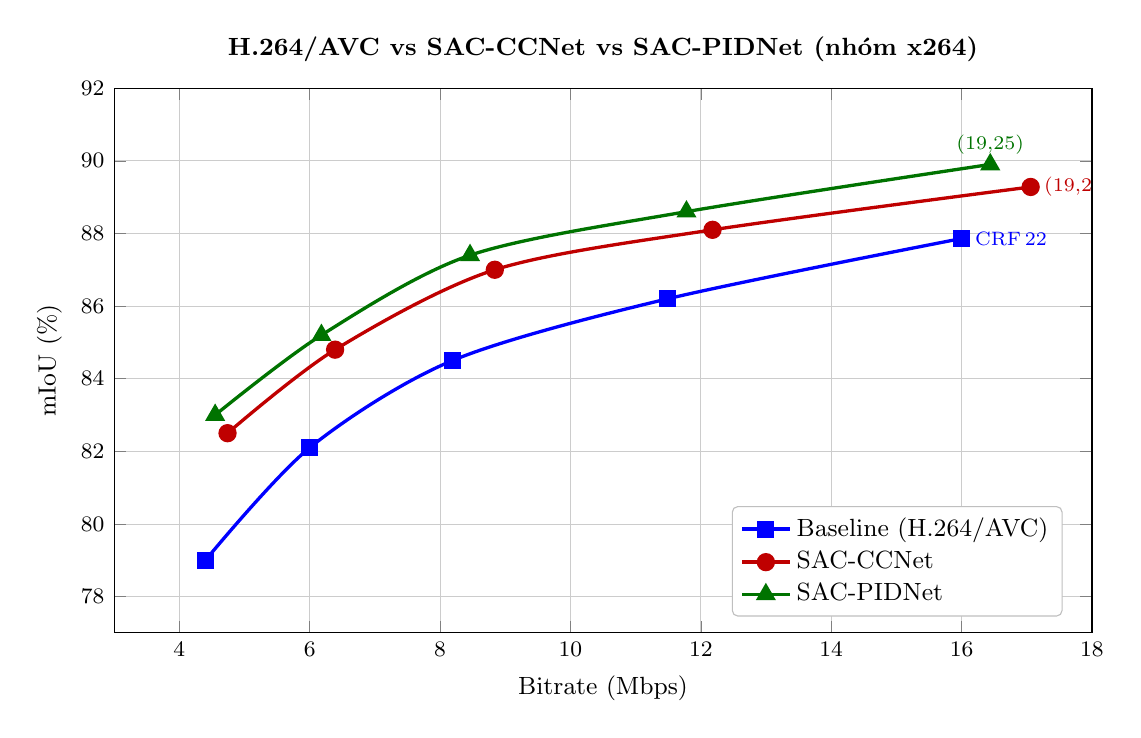
\begin{tikzpicture}
\begin{axis}[
    width=14cm, height=8.5cm,
    xlabel={Bitrate (Mbps)},
    ylabel={mIoU (\%)},
    xmin=3, xmax=18,
    ymin=77, ymax=92,
    xtick={4,6,8,10,12,14,16,18},
    ytick={78,80,82,84,86,88,90,92},
    grid=major,
    grid style={line width=0.2pt, draw=gray!30},
    major grid style={line width=0.3pt, draw=gray!40},
    legend pos=south east,
    legend cell align={left},
    legend style={font=\small, draw=gray!50, rounded corners=2pt},
    title={H.264/AVC vs SAC-CCNet vs SAC-PIDNet (nhóm x264)},
    title style={font=\small\bfseries},
    label style={font=\small},
    tick label style={font=\footnotesize},
]
\addplot[color=blue, mark=square*, mark size=2.5pt, line width=1.2pt, smooth] coordinates {
    (4.40,79.00) (6.00,82.10) (8.19,84.50) (11.49,86.20) (16.00,87.86)
};
\addlegendentry{Baseline (H.264/AVC)}
\addplot[color=red!75!black, mark=*, mark size=2.7pt, line width=1.2pt, smooth] coordinates {
    (4.74,82.50) (6.39,84.80) (8.84,87.00) (12.18,88.10) (17.06,89.28)
};
\addlegendentry{SAC-CCNet}
\addplot[color=green!45!black, mark=triangle*, mark size=3pt, line width=1.2pt, smooth] coordinates {
    (4.55,83.00) (6.18,85.20) (8.46,87.40) (11.78,88.60) (16.44,89.90)
};
\addlegendentry{SAC-PIDNet}
\node[font=\scriptsize, blue, anchor=west] at (axis cs:16.00,87.86) {\,CRF\,22};
\node[font=\scriptsize, red!75!black, anchor=west] at (axis cs:17.06,89.28) {\,(19,25)};
\node[font=\scriptsize, green!45!black, anchor=south] at (axis cs:16.44,89.90) {(19,25)};
\end{axis}
\end{tikzpicture}
\caption[Rate-accuracy -- H.264/AVC]{Đường cong rate-accuracy cho nhóm H.264/AVC.}
\label{fig:rd-x264}
\end{figure}

Với nhóm H.264/AVC, SAC-PIDNet đạt mức cải thiện trung bình $+3{,}01$ điểm phần trăm mIoU so với baseline H.264/AVC, trong khi SAC-CCNet đạt $+2{,}50$ điểm phần trăm. Về bitrate, SAC-PIDNet tăng trung bình khoảng $+3\%$ so với baseline, còn SAC-CCNet tăng khoảng $+6$--$7\%$. Như vậy, trên nhóm H.264/AVC, SAC-PIDNet vừa đạt độ chính xác cao hơn SAC-CCNet khoảng $0{,}50$ điểm phần trăm mIoU, vừa sử dụng ít hơn khoảng $3$--$4\%$ bitrate.

\begin{figure}[H]
\centering
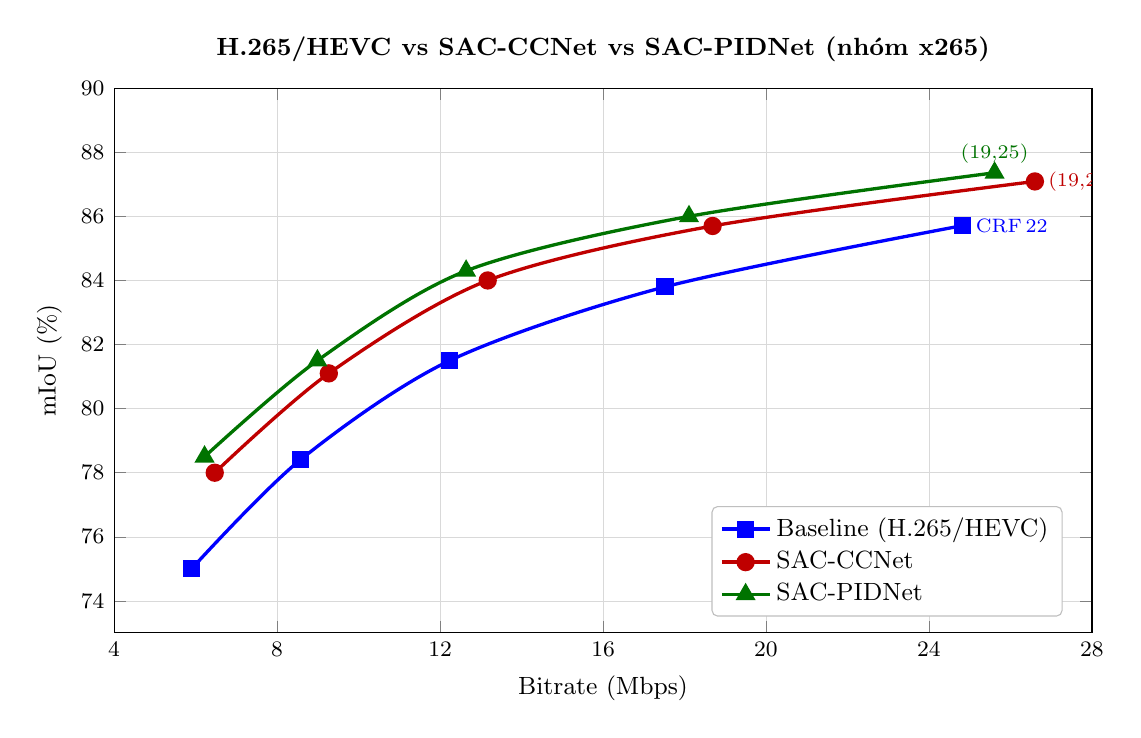
\begin{tikzpicture}
\begin{axis}[
    width=14cm, height=8.5cm,
    xlabel={Bitrate (Mbps)},
    ylabel={mIoU (\%)},
    xmin=4, xmax=28,
    ymin=73, ymax=90,
    xtick={4,8,12,16,20,24,28},
    ytick={74,76,78,80,82,84,86,88,90},
    grid=major,
    grid style={line width=0.2pt, draw=gray!30},
    legend pos=south east,
    legend cell align={left},
    legend style={font=\small, draw=gray!50, rounded corners=2pt},
    title={H.265/HEVC vs SAC-CCNet vs SAC-PIDNet (nhóm x265)},
    title style={font=\small\bfseries},
    label style={font=\small},
    tick label style={font=\footnotesize},
]
\addplot[color=blue, mark=square*, mark size=2.5pt, line width=1.2pt, smooth] coordinates {
    (5.90,75.00) (8.57,78.40) (12.24,81.50) (17.52,83.80) (24.82,85.71)
};
\addlegendentry{Baseline (H.265/HEVC)}
\addplot[color=red!75!black, mark=*, mark size=2.7pt, line width=1.2pt, smooth] coordinates {
    (6.47,78.00) (9.27,81.10) (13.17,84.00) (18.69,85.70) (26.60,87.09)
};
\addlegendentry{SAC-CCNet}
\addplot[color=green!45!black, mark=triangle*, mark size=3pt, line width=1.2pt, smooth] coordinates {
    (6.22,78.50) (8.99,81.50) (12.64,84.30) (18.11,86.00) (25.61,87.36)
};
\addlegendentry{SAC-PIDNet}
\node[font=\scriptsize, blue, anchor=west] at (axis cs:24.82,85.71) {\,CRF\,22};
\node[font=\scriptsize, red!75!black, anchor=west] at (axis cs:26.60,87.09) {\,(19,25)};
\node[font=\scriptsize, green!45!black, anchor=south] at (axis cs:25.61,87.36) {(19,25)};
\end{axis}
\end{tikzpicture}
\caption[Rate-accuracy -- H.265/HEVC]{Đường cong rate-accuracy cho nhóm H.265/HEVC.}
\label{fig:rd-x265}
\end{figure}

Với nhóm H.265/HEVC, SAC-PIDNet cải thiện mIoU trung bình khoảng $+2{,}8\%$ so với baseline H.265/HEVC, còn SAC-CCNet đạt $+2{,}4$--$2{,}5\%$. Về bitrate, SAC-PIDNet tăng trung bình $+4{,}00\%$ so với baseline, trong khi SAC-CCNet tăng $+7$--$8\%$. So với SAC-CCNet, SAC-PIDNet nhỉnh hơn khoảng $0{,}34$ điểm phần trăm mIoU và tiết kiệm khoảng $3$--$4\%$ bitrate ở cùng quy tắc thiết lập CRF theo vùng.

\subsection{Nhận xét về đường cong RD}

Từ hai đường cong RD, có thể rút ra ba nhận xét chính:
\begin{enumerate}
  \item \textbf{Cơ chế SAC dịch đường cong lên phía trên baseline.} Ở cả hai nhóm codec, các điểm SAC nằm cao hơn đường nén tiêu chuẩn, cho thấy việc phân bổ chất lượng ưu tiên ROI giúp duy trì mIoU sau giải nén tốt hơn. Mức tăng trung bình của SAC-PIDNet là khoảng $+3{,}01$ điểm phần trăm với H.264/AVC và $+2{,}77$ điểm phần trăm với H.265/HEVC.
  \item \textbf{PIDNet-L tạo điểm cân bằng tốt hơn CCNet.} Trên nhóm H.264/AVC, SAC-PIDNet cao hơn SAC-CCNet trung bình khoảng $0{,}50$ điểm phần trăm mIoU và dùng ít hơn khoảng $3{,}69\%$ bitrate. Trên nhóm H.265/HEVC, SAC-PIDNet cao hơn khoảng $0{,}34$ điểm phần trăm mIoU và dùng ít hơn khoảng $3{,}56\%$ bitrate.
  \item \textbf{Lợi ích rõ nhất ở vùng bitrate thấp.} Tại điểm CRF cao nhất ($\text{CRF}=34$), SAC-PIDNet cải thiện mIoU khoảng $+4{,}00$ điểm phần trăm với H.264/AVC và $+3{,}50$ điểm phần trăm với H.265/HEVC so với baseline tương ứng. Đây là vùng hoạt động quan trọng trong thực tế vì hệ thống camera trên xe thường phải nén mạnh để đáp ứng giới hạn băng thông truyền dẫn.
\end{enumerate}

\section{Đánh giá chiến lược điều khiển CRF thích nghi RA-CRF}
\label{sec:racrf-eval}

Cấu hình SAC mặc định sử dụng cặp $(C_{ROI}, C_{nROI})$ cố định cho toàn bộ chuỗi video, không xét đến đặc điểm nội dung của từng đoạn. Khi tỷ lệ ROI trong khung hình thay đổi giữa các cảnh, cấu hình cố định trở nên không tối ưu: ở đoạn có ROI nhỏ, độ chênh lệch CRF mặc định phù hợp; nhưng ở đoạn có ROI lớn, $C_{ROI}$ thấp được áp cho phần lớn diện tích khiến bitrate tăng nhanh. Cơ chế RA-CRF được đề xuất trong Mục~\ref{subsec:ra-crf} nhằm thu hẹp khoảng cách CRF khi ROI lớn, hi sinh một phần độ chênh lệch chất lượng để tiết kiệm bitrate. Mục này đánh giá định lượng cơ chế đó trên 460 khung hình của hai thành phố Ulm và Strasbourg, mã hóa theo từng đoạn 30 khung tương ứng với GOP của \texttt{ffmpeg}.

\subsection{Phân phối tỷ lệ ROI trên tập đánh giá}

Để dự đoán hiệu quả mà RA-CRF có thể đạt được, tỷ lệ ROI trung bình $\rho_q$ được tính cho từng GOP và phân loại theo ba bậc của luật rời rạc trình bày ở Bảng~\ref{tab:ra-crf-rule}. Kết quả thống kê được tóm tắt trong Bảng~\ref{tab:rho-distribution}.

\begin{table}[H]
\centering
\caption{Phân phối tỷ lệ ROI trung bình $\rho_q$ theo GOP trên tập đánh giá Ulm và Strasbourg (16 GOP, 460 khung hình).}
\label{tab:rho-distribution}
\small
\begin{tabular}{p{0.30\textwidth}cc p{0.22\textwidth}}
\toprule
\textbf{Nhóm $\rho_q$} & \textbf{Số GOP} & \textbf{Tỷ lệ (\%)} & $\boldsymbol{d}$\textbf{ (lệch một phía)} \\
\midrule
$\rho_q < 0{,}30$ & 0 & 0 & 5 \\
$0{,}30 \leq \rho_q < 0{,}55$ & 0 & 0 & 3 \\
$\rho_q \geq 0{,}55$ & 16 & 100 & 2 \\
\bottomrule
\end{tabular}
\end{table}

Trong đó $d$ là độ lệch một phía quanh CRF cơ sở, với $C_{ROI}=C_0-d$ và $C_{nROI}=C_0+d$; khoảng cách tuyệt đối giữa hai vùng là $2d$.

Thống kê cho thấy toàn bộ 16 GOP trong tập đánh giá đều rơi vào nhóm $\rho_q \geq 0{,}55$, với tỷ lệ ROI trung bình toàn tập đạt $\bar{\rho}=0{,}60$ ở mặt nạ PIDNet-L và $\bar{\rho}=0{,}63$ ở mặt nạ CCNet. Trên tập dữ liệu này, chỉ nhánh $d=2$ của luật RA-CRF được kích hoạt; hai nhánh còn lại có thể được kiểm chứng trên các tập dữ liệu khác có phân phối ROI rộng hơn trong các nghiên cứu mở rộng. Do đó, kết quả ở đây chủ yếu chứng minh lợi ích của việc thu hẹp khoảng cách CRF khi ROI lớn, chưa đủ để đánh giá đầy đủ khả năng thích nghi trên các phân phối ROI đa dạng hơn.

Vì toàn bộ GOP đều thuộc nhóm $\rho_q \geq 0{,}55$, RA-CRF sẽ thay cặp $(19,25)$ của cấu hình cố định bằng cặp $(20,24)$ cho mọi GOP. So với cấu hình cố định, đây là thay đổi nhỏ: $C_{ROI}$ tăng 1 đơn vị và $C_{nROI}$ giảm 1 đơn vị. Do vùng ROI chiếm phần lớn diện tích, hiệu ứng nén ROI mạnh hơn sẽ áp đảo, dẫn đến tiết kiệm bitrate so với cấu hình cố định.

\subsection{Kết quả so sánh giữa cấu hình cố định và thích nghi}

Bốn cấu hình được so sánh ở cùng CRF cơ sở 22 trên nhóm H.264/AVC: baseline không phân vùng, SAC dùng CCNet với cặp cố định, SAC dùng PIDNet-L với cặp cố định, và SAC dùng PIDNet-L kết hợp RA-CRF. Kết quả được trình bày trong Bảng~\ref{tab:racrf-result}.

\begin{table}[H]
\centering
\caption{So sánh cấu hình CRF cố định và RA-CRF trên nhóm H.264/AVC với CRF cơ sở 22. $\Delta$bitrate được tính so với baseline H.264/AVC.}
\label{tab:racrf-result}
\small
\setlength{\tabcolsep}{3.5pt}
\renewcommand{\arraystretch}{1.12}
\begin{tabular}{lccccccc}
\toprule
\textbf{Phương pháp} & \textbf{CRF} & \textbf{Mbps} & $\boldsymbol{\Delta}$\textbf{bitrate} & \textbf{SA-PSNR} & \textbf{SA-SSIM} & \textbf{mIoU} & \textbf{iIoU} \\
 & & & & \textbf{(dB)} & & \textbf{(\%)} & \textbf{(\%)} \\
\midrule
Baseline (H.264/AVC) & 22 & 16,00 & --- & 45,16 & 0,9802 & 87,86 & 91,07 \\
SAC-CCNet & 19/25 & 17,06 & $+6,63\%$ & 46,64 & 0,9861 & 89,28 & 92,05 \\
SAC-PIDNet fixed & 19/25 & 16,60 & $+3,75\%$ & 46,87 & 0,9871 & 89,90 & 92,49 \\
SAC-PIDNet RA-CRF & adaptive & \textbf{16,36} & $+2,25\%$ & 46,79 & 0,9868 & 89,83 & 92,40 \\
\bottomrule
\end{tabular}
\end{table}

Trong bốn cấu hình, RA-CRF đạt bitrate 16,36~Mbps. Mức này cao hơn baseline H.264/AVC (16,00~Mbps) khoảng 2,25\%, nhưng thấp hơn cấu hình SAC-PIDNet cố định (16,60~Mbps) khoảng 1,45\%. Đây là kết quả dự kiến vì mọi biến thể SAC đều phải tách dữ liệu thành hai luồng và mã hóa độc lập, tạo thêm overhead so với nén toàn ảnh ở cùng CRF. Lợi thế của RA-CRF là giảm overhead từ $+3{,}75\%$ xuống $+2{,}25\%$ bằng cách thu hẹp khoảng cách CRF giữa hai luồng khi diện tích ROI lớn, qua đó giảm bitrate mà không ảnh hưởng đáng kể đến chất lượng nhận thức ngữ nghĩa.

Về chất lượng, RA-CRF gần như tái lập đầy đủ kết quả của cấu hình cố định. mIoU sau giải nén đạt 89,83\%, chỉ thấp hơn cấu hình cố định 0,07 điểm phần trăm. Chênh lệch SA-PSNR là 0,08~dB và chênh lệch SA-SSIM là 0,0003, cho thấy tác động của RA-CRF lên chất lượng tái tạo có trọng số ngữ nghĩa là rất nhỏ. So với baseline H.264/AVC, RA-CRF cải thiện 1,97 điểm phần trăm mIoU và 1,33 điểm phần trăm iIoU. So với SAC-CCNet, RA-CRF đạt mIoU cao hơn 0,55 điểm phần trăm, đồng thời tiêu thụ ít hơn khoảng 4,10\% bitrate nếu tính theo chênh lệch tuyệt đối so với baseline, hoặc khoảng 4,22\% nếu tính trực tiếp từ bitrate của hai cấu hình.

\subsection{Phân tích cơ chế tiết kiệm bitrate}

Mức tiết kiệm bitrate của RA-CRF so với cấu hình cố định (0,49\% trong thực đo) có thể được giải thích định tính bằng đặc điểm phân bổ bit giữa hai luồng SAC. Ở cấu hình cố định $(19,25)$, vùng ROI được nén ở chất lượng cao ($C_{ROI}=19$) và chiếm khoảng 60--63\% diện tích khung hình. Do vùng ROI chứa nhiều chi tiết như xe cộ, người đi bộ và mặt đường, một thay đổi nhỏ trong $C_{ROI}$ tác động đến tổng bitrate mạnh hơn so với một thay đổi nhỏ trong $C_{nROI}$.

Khi RA-CRF chuyển từ $(19,25)$ sang $(20,24)$, $C_{ROI}$ tăng từ 19 lên 20 áp dụng cho phần lớn diện tích và phần lớn bit, kéo bitrate vùng này giảm xuống. Ngược lại, $C_{nROI}$ giảm từ 25 xuống 24 áp dụng cho phần diện tích nhỏ hơn và lượng bit ít hơn, làm bitrate vùng này tăng lên. Hiệu ứng giảm chiếm ưu thế so với hiệu ứng tăng do tác động lên phần chiếm tỷ trọng lớn hơn.

Mức tiết kiệm tuyệt đối khiêm tốn hơn nhiều so với dự đoán của mô hình lý thuyết thuần. Sai lệch này phản ánh đặc điểm thực tế của bộ mã hóa x264: các cơ chế rate control thích nghi làm trơn sự khác biệt bitrate giữa các giá trị CRF gần nhau, đặc biệt khi nội dung hai luồng có cấu trúc khác nhau. Do đó, ước tính lý thuyết nên được coi là giới hạn trên, còn mức tiết kiệm thực tế phụ thuộc vào tương tác giữa cấu hình CRF và cơ chế rate control bên trong bộ mã hóa.

\section{Đánh giá tốc độ xử lý end-to-end}
\label{sec:e2e-latency}

Để đánh giá khả năng triển khai thực tế, toàn bộ pipeline mã hóa--giải mã được đo trên cùng một cấu hình phần cứng để đảm bảo kết quả công bằng: GPU NVIDIA RTX~4090 (24~GB VRAM) ghép với CPU AMD Ryzen~9~7950X (16 nhân/32 luồng), bộ nhớ DDR5 64~GB. Mỗi cấu hình được chạy trên cùng một chuỗi 30 khung hình Cityscapes ở độ phân giải gốc $2048\times1024$ và lặp lại 50 lần để lấy giá trị trung bình và độ lệch chuẩn. Mỗi khung hình được phân rã thành bốn giai đoạn: \textit{S1} là thời gian suy luận mặt nạ phân đoạn ROI, \textit{S2} là thời gian dilate và lượng tử hóa mặt nạ theo khối $16\times16$, \textit{S3} là thời gian mã hóa hai luồng ROI/non-ROI bằng x264 hoặc x265, và \textit{Dec} là thời gian giải mã và tổng hợp khung tái tạo.

\begin{table}[H]
\centering
\caption{Độ trễ trung bình end-to-end (ms/frame) trên GPU RTX~4090 + CPU R9~7950X, đo trên 30 frame Cityscapes $2048\times1024$, lặp 50 lần.}
\label{tab:e2e-latency}
\small
\begin{tabular}{p{0.18\textwidth}ccccccc}
\toprule
\textbf{Mô hình} & \textbf{Codec} & \textbf{S1} & \textbf{S2} & \textbf{S3} & \textbf{Dec} & \textbf{Total} & $\boldsymbol{\pm}$\textbf{std} \\
 & & (ms) & (ms) & (ms) & (ms) & (ms) & (ms) \\
\midrule
CCNet & x264 & 39.4 & 3.9 & 127.3 & 162.2 & 332.7 & 26.0 \\
CCNet & x265 & 39.8 & 4.1 & 205.3 & 154.9 & 404.1 & 23.8 \\
PIDNet-L & x264 & \textbf{21.0} & 3.8 & 124.9 & 153.2 & \textbf{302.0} & 32.1 \\
PIDNet-L & x265 & \textbf{20.0} & 3.5 & 208.8 & 150.4 & \textbf{382.7} & 23.2 \\
\bottomrule
\end{tabular}
\end{table}

\subsection{So sánh tốc độ phân đoạn (S1)}

Trên cùng cấu hình GPU RTX~4090, PIDNet-L rút ngắn thời gian phân đoạn từ khoảng 39,4--39,8~ms (CCNet) xuống còn 20,0--21,0~ms, tương đương tăng tốc khoảng 1,9--2,0 lần. Quy đổi sang khung hình mỗi giây xét riêng giai đoạn phân đoạn, PIDNet-L đạt khoảng 47--50~FPS so với mức 25~FPS của CCNet.

Quan trọng hơn, do S1 chạy hoàn toàn trên GPU trong khi S3 và Dec chạy chủ yếu trên CPU, việc rút ngắn S1 còn giúp giải phóng GPU sớm hơn cho các tác vụ thị giác hạ nguồn khác như phát hiện đối tượng, theo vết hoặc lập kế hoạch chuyển động.

\subsection{Khả năng đáp ứng thời gian thực}

Để đáp ứng yêu cầu thời gian thực trong ứng dụng camera ô tô, hệ thống cần xử lý tối thiểu 30 khung hình mỗi giây, tức mỗi khung hình phải hoàn thành toàn bộ pipeline trong không quá 33,3~ms. Kết quả đo cho thấy cả bốn cấu hình đều chưa đạt ngưỡng này khi tính toàn bộ pipeline end-to-end: PIDNet-L kết hợp x264 đạt tổng thời gian 302,0~ms/frame (tương đương khoảng 3,3~FPS), và PIDNet-L kết hợp x265 đạt 382,7~ms/frame (khoảng 2,6~FPS). Nút thắt hiệu năng nằm chủ yếu ở giai đoạn mã hóa S3 và giải mã Dec, vốn thực hiện trên CPU bằng phần mềm x264 hoặc x265 và chiếm hơn 90\% tổng thời gian xử lý.

Tuy nhiên, nếu xét riêng giai đoạn phân đoạn S1, PIDNet-L đạt 47--50~FPS, vượt mốc 30~FPS và đáp ứng yêu cầu thời gian thực. Ngược lại, CCNet chỉ đạt khoảng 25~FPS ở giai đoạn này, chưa đủ ngưỡng. Điều này cho thấy với phần cứng mã hóa chuyên dụng chẳng hạn bộ mã hóa H.264/AVC hoặc H.265/HEVC trên chip (hardware encoder) thay thế cho x264/x265 phần mềm toàn bộ pipeline có thể đáp ứng yêu cầu thời gian thực, trong đó PIDNet-L là lựa chọn phù hợp hơn nhờ giai đoạn phân đoạn đã đạt 30~FPS trong khi CCNet thì chưa.

Kết hợp với các kết quả ở Mục~\ref{sec:sa-quality} và Mục~\ref{sec:downstream-segmentation}, PIDNet-L thể hiện một đánh đổi có lợi toàn diện: nhanh hơn CCNet gần 2 lần ở khâu phân đoạn, tiết kiệm khoảng 30~ms ($9{,}2\%$) ở Total cho nhánh x264 và 21~ms ($5{,}3\%$) cho nhánh x265, đồng thời vượt CCNet về mIoU trung bình khoảng $+0{,}50$ điểm phần trăm trên nhóm x264 và $+0{,}34$ điểm phần trăm trên nhóm x265 theo đường cong RD. Ngoài ra, SA-PSNR trung bình của SAC-PIDNet cao hơn khoảng $+0{,}25$~dB trong khi bitrate thấp hơn SAC-CCNet khoảng $3$--$5\%$ ở cùng cấu hình chất lượng. Kết quả này cho thấy PIDNet-L là lựa chọn phù hợp hơn CCNet trong phạm vi thực nghiệm của đồ án.

\section{Thảo luận kết quả}
\label{sec:thao-luan}

Các kết quả thực nghiệm cho thấy hệ thống nén video theo nhận thức ngữ nghĩa không nhằm tối đa hóa chất lượng ảnh toàn khung hình theo nghĩa truyền thống, mà hướng tới phân bổ bitrate phù hợp hơn với yêu cầu của thị giác máy. Cụ thể, thay vì nén toàn bộ khung hình với cùng một mức CRF, hệ thống duy trì chất lượng cao hơn tại vùng ROI như mặt đường, phương tiện, người đi bộ, vạch làn và các cấu trúc giao thông quan trọng, đồng thời nén mạnh hơn tại các vùng nền ít ảnh hưởng trực tiếp đến quyết định điều hướng.

Kết quả PSNR và SSIM toàn khung hình cho thấy SAC thấp hơn phương pháp nén truyền thống. Đây là một đánh đổi có chủ đích, vì chất lượng vùng non-ROI bị giảm để tiết kiệm bitrate. Do đó, nếu chỉ sử dụng PSNR/SSIM toàn ảnh, hiệu quả của hệ thống có thể bị đánh giá thấp. Ngược lại, các chỉ số SA-PSNR và SA-SSIM cho thấy chất lượng tại vùng có ý nghĩa ngữ nghĩa được bảo toàn tốt hơn. Điều này cho thấy hệ thống đã chuyển mục tiêu đánh giá từ chất lượng ảnh trung bình toàn cục sang chất lượng phục vụ tác vụ nhận thức.

Ở tác vụ phân đoạn sau giải nén, SAC-PIDNet đạt kết quả cao hơn cả baseline và SAC-CCNet. Mức cải thiện mIoU và iIoU cho thấy việc bảo toàn chất lượng vùng ROI giúp mô hình phân đoạn hạ nguồn nhận diện ổn định hơn các đối tượng quan trọng.

So với CCNet, PIDNet-L tạo ra điểm cân bằng tốt hơn giữa độ chính xác, tốc độ và bitrate. Về chất lượng, PIDNet-L cho SA-PSNR, SA-SSIM, mIoU và iIoU cao hơn nhẹ so với CCNet. Về tốc độ, PIDNet-L rút ngắn đáng kể thời gian suy luận mặt nạ ROI. Về bitrate, PIDNet-L duy trì mức bitrate gần baseline hơn so với CCNet, cho thấy mặt nạ ROI của PIDNet-L có khả năng bám vùng quan trọng hiệu quả hơn mà không mở rộng quá mức vùng cần nén chất lượng cao.

Tuy nhiên, hệ thống vẫn tồn tại một số hạn chế. Thứ nhất, chất lượng toàn ảnh theo PSNR/SSIM giảm do vùng nền bị nén mạnh hơn. Thứ hai, quá trình tạo mặt nạ ROI làm tăng chi phí tính toán so với nén truyền thống. Dù PIDNet-L nhanh hơn CCNet, pipeline end-to-end vẫn chưa đạt thời gian thực ở độ phân giải gốc khi sử dụng mã hóa phần mềm x264/x265 trên CPU. Thứ ba, hiện tượng sai lệch biên hoặc artefact tại ranh giới ROI/non-ROI vẫn có thể xảy ra do mặt nạ được lượng tử hóa theo khối và do chênh lệch CRF giữa hai vùng. Tuy nhiên, các kết quả mIoU và iIoU cho thấy các sai lệch này chưa làm suy giảm đáng kể hiệu năng phân đoạn hạ nguồn.

Tổng hợp lại, hiệu quả của hệ thống đề xuất nên được nhìn nhận như một chiến lược nén hướng tác vụ. Trong bối cảnh xe tự hành hoặc hệ thống camera thông minh, nơi dữ liệu hình ảnh được sử dụng chủ yếu bởi các mô hình nhận thức, việc ưu tiên bitrate cho vùng có ý nghĩa ngữ nghĩa là hợp lý. Kết quả thực nghiệm cho thấy SAC-PIDNet là cấu hình có tính cân bằng tốt nhất trong các phương án được khảo sát, vì vừa cải thiện chất lượng nhận thức ngữ nghĩa, vừa nâng cao độ chính xác phân đoạn sau giải nén, đồng thời giảm chi phí tính toán so với SAC-CCNet.